\section{The Effect of Number of Variants on SQL Generators}
\label{sec:exp-vars}


%\begin{wrapfigure}{r}{0.5\linewidth}
%\centering
%\rule{0.9\linewidth}{0.75\linewidth}
%\caption{Dummy figure.}
%\label{fig:myfig}
%\end{wrapfigure}
%\blindtext


\begin{figure}
\centering
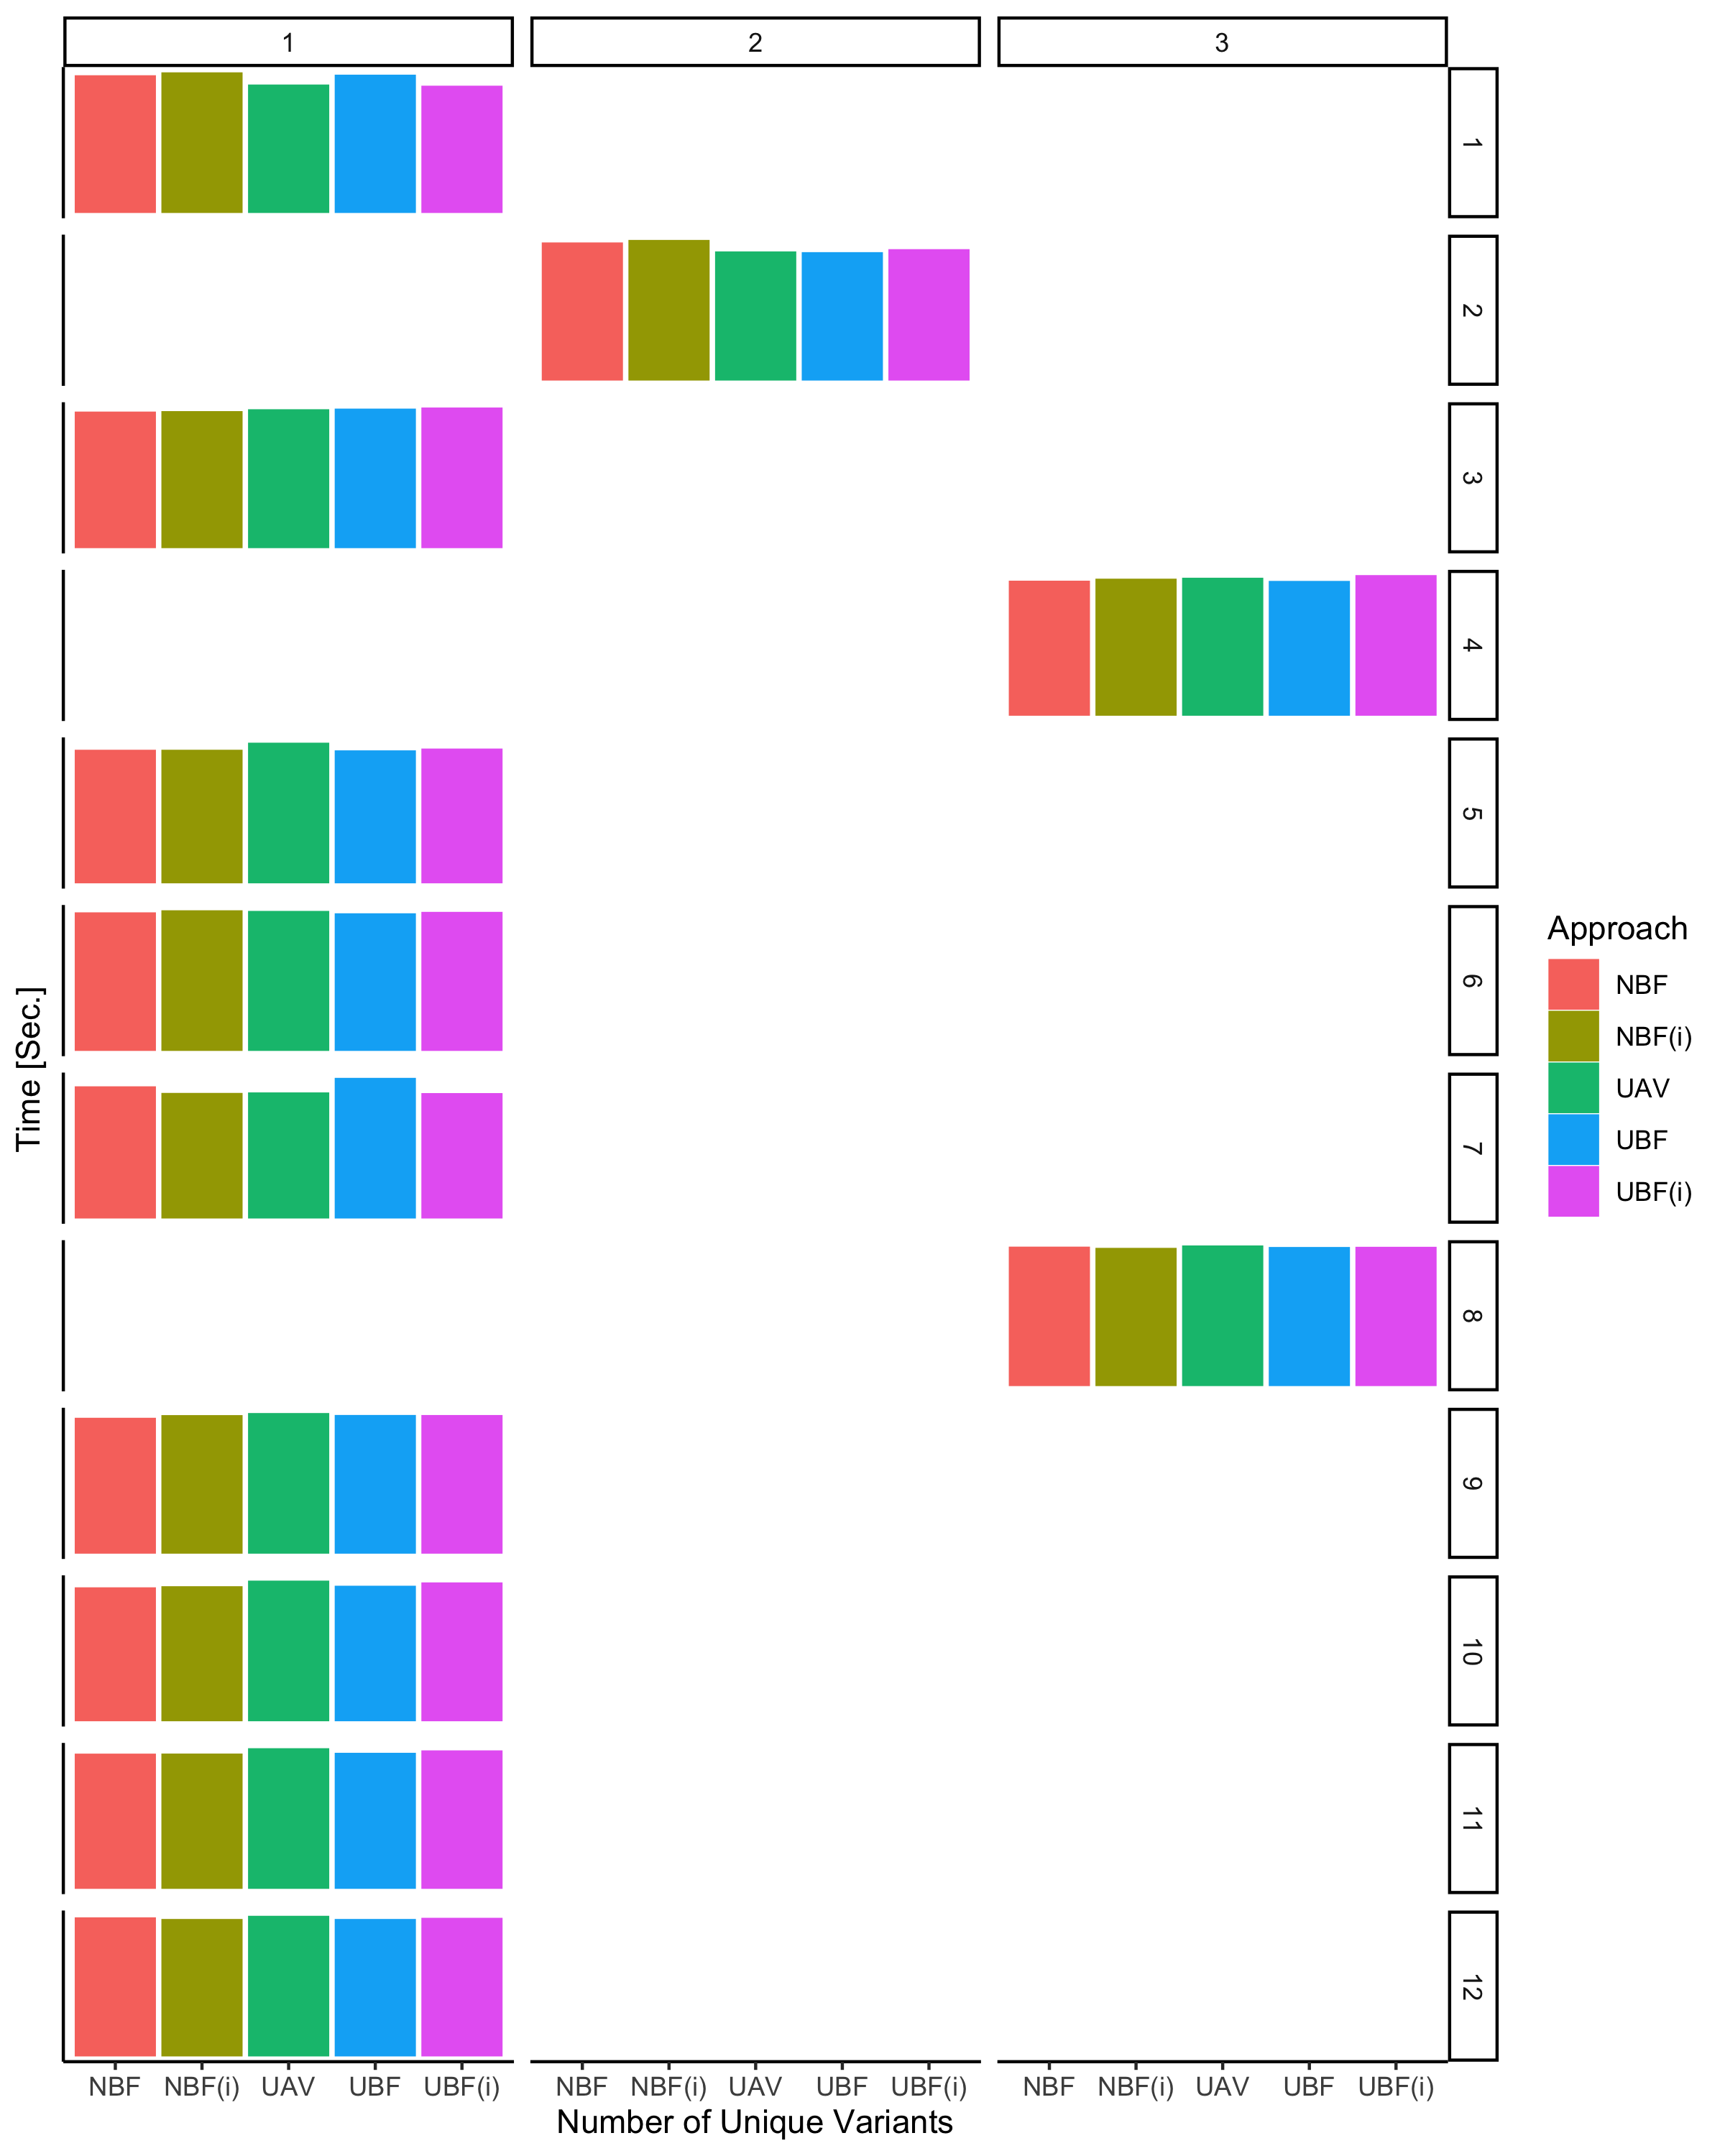
\includegraphics[scale = 0.1] {figs/plots/emp-comp-var.png}
\caption[blah]{blah}
\label{fig:-}
\end{figure}

\begin{figure}
\centering
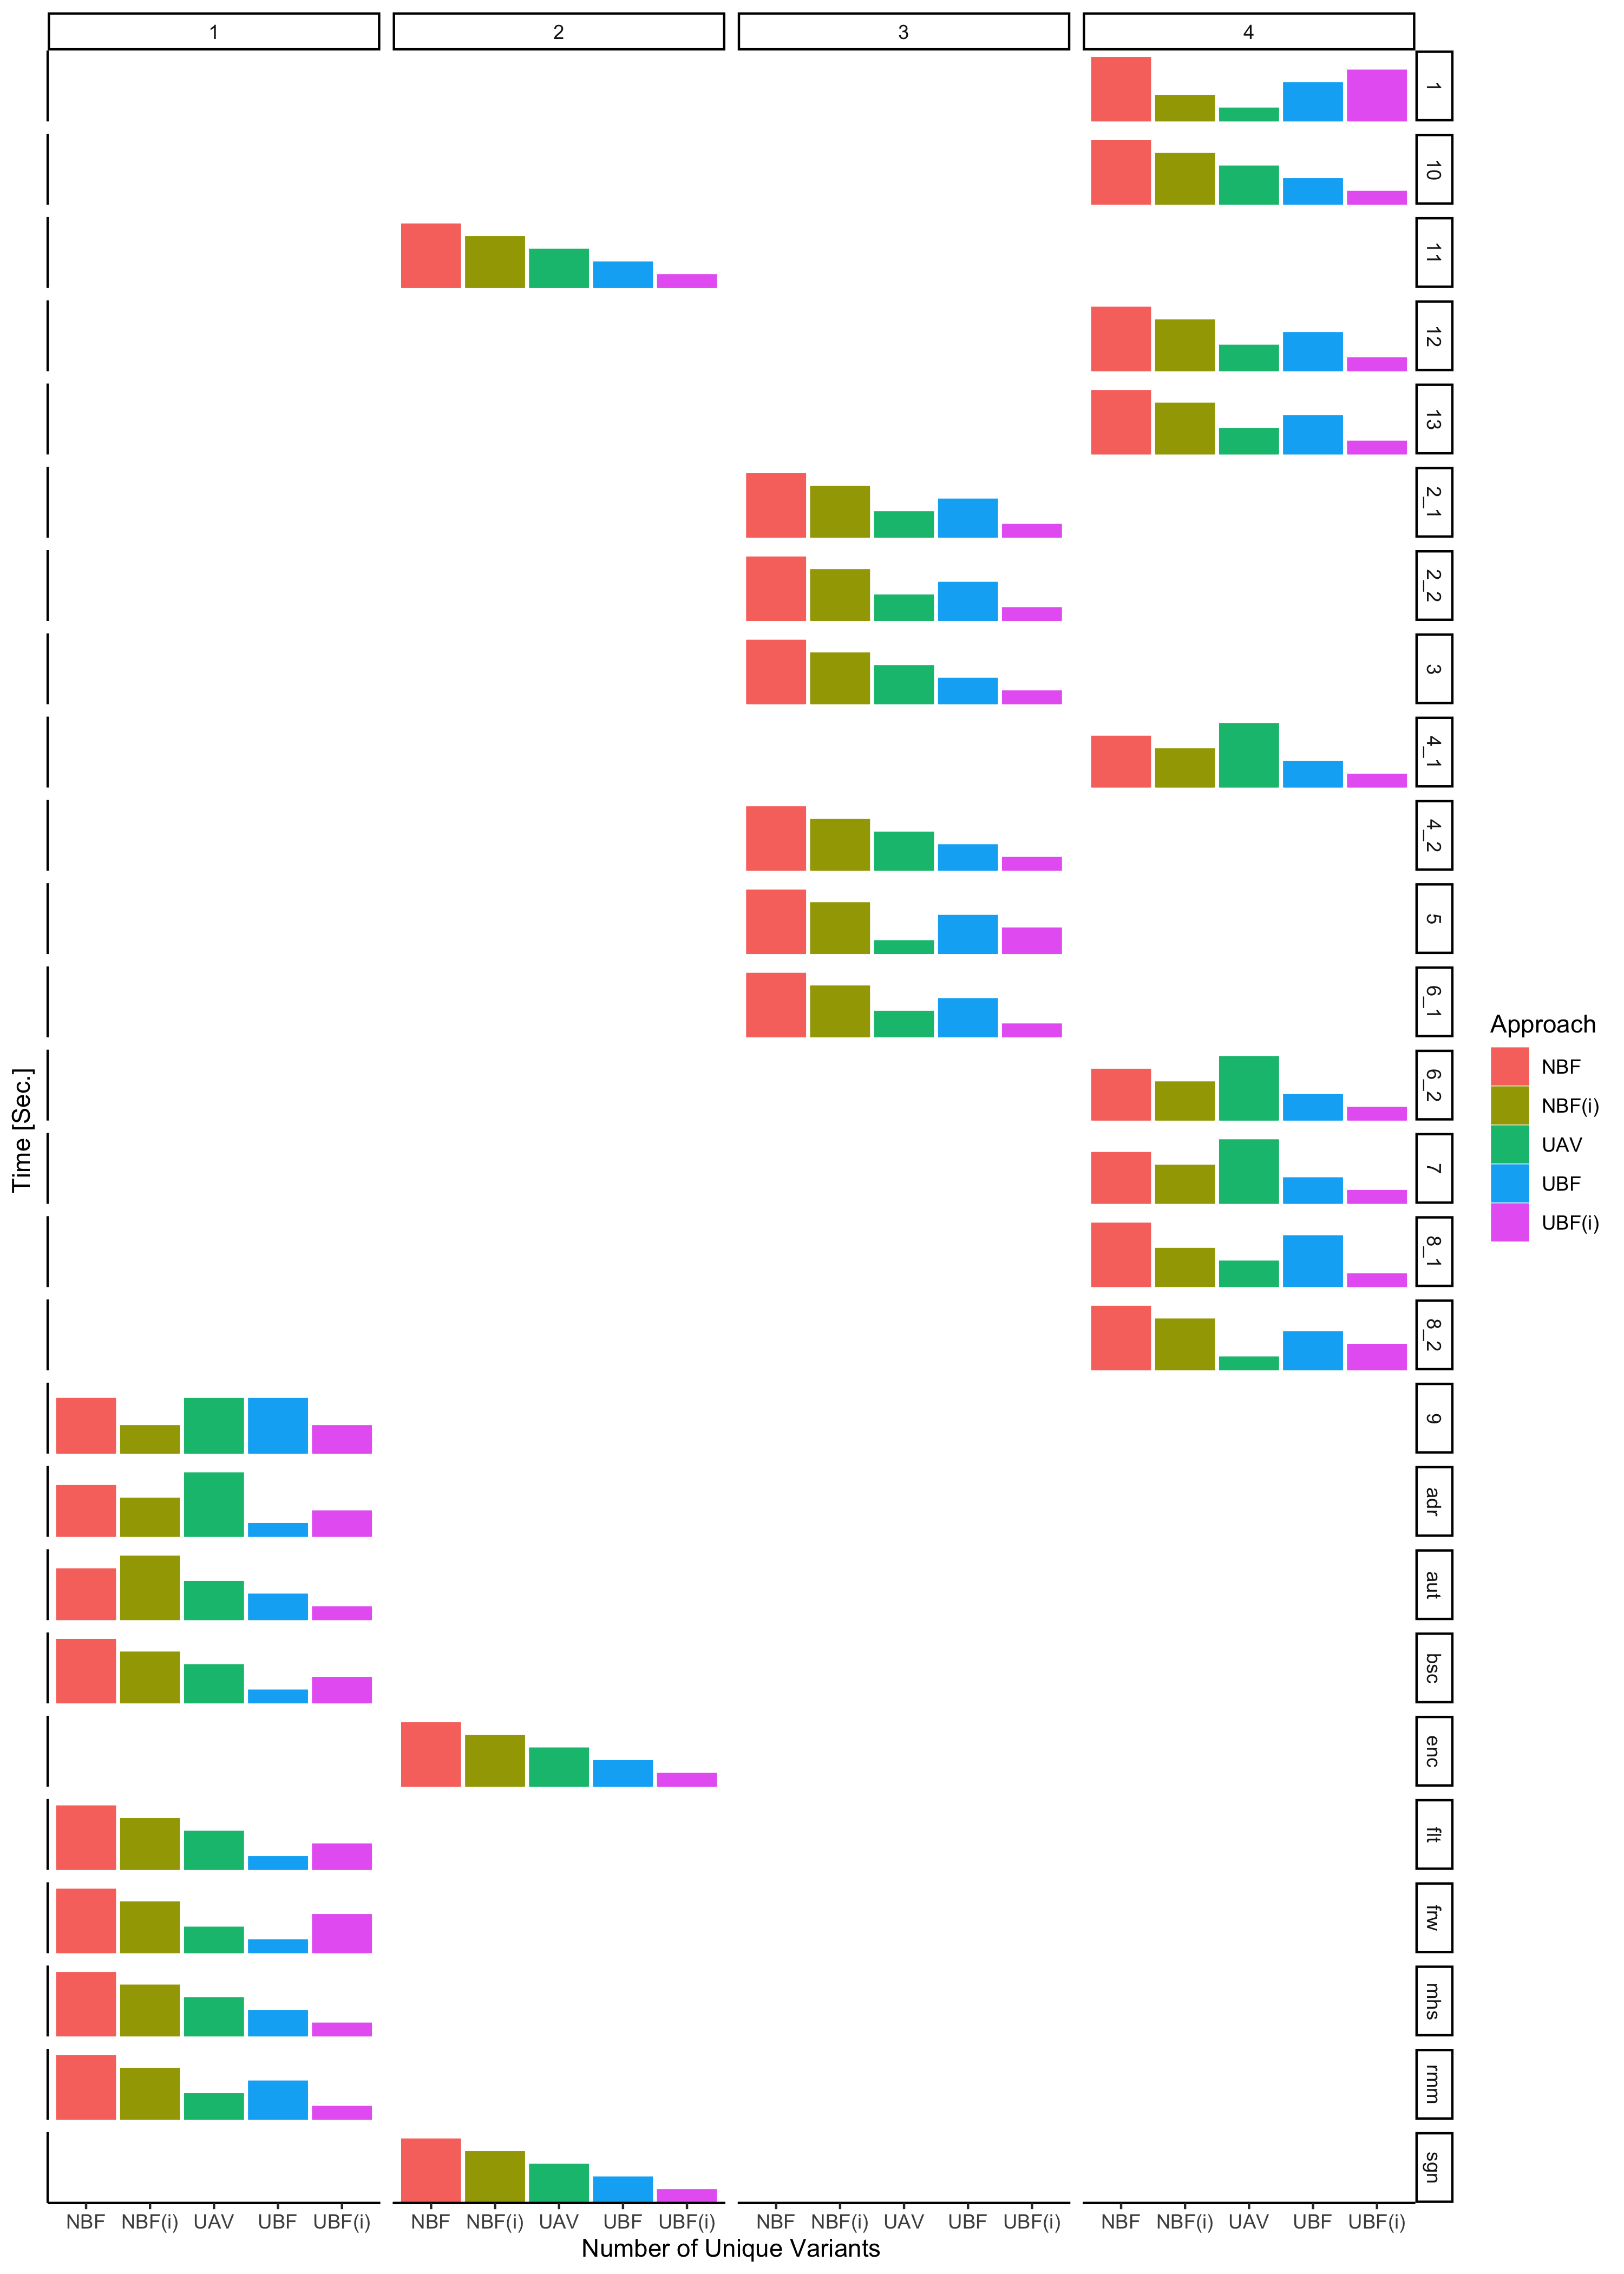
\includegraphics[scale=0.1] {figs/plots/enron-comp-var.png}
\caption[blah]{blah}
\label{fig:-}
\end{figure}


\begin{figure}
\begin{subfigure}{.5\linewidth}
\centering
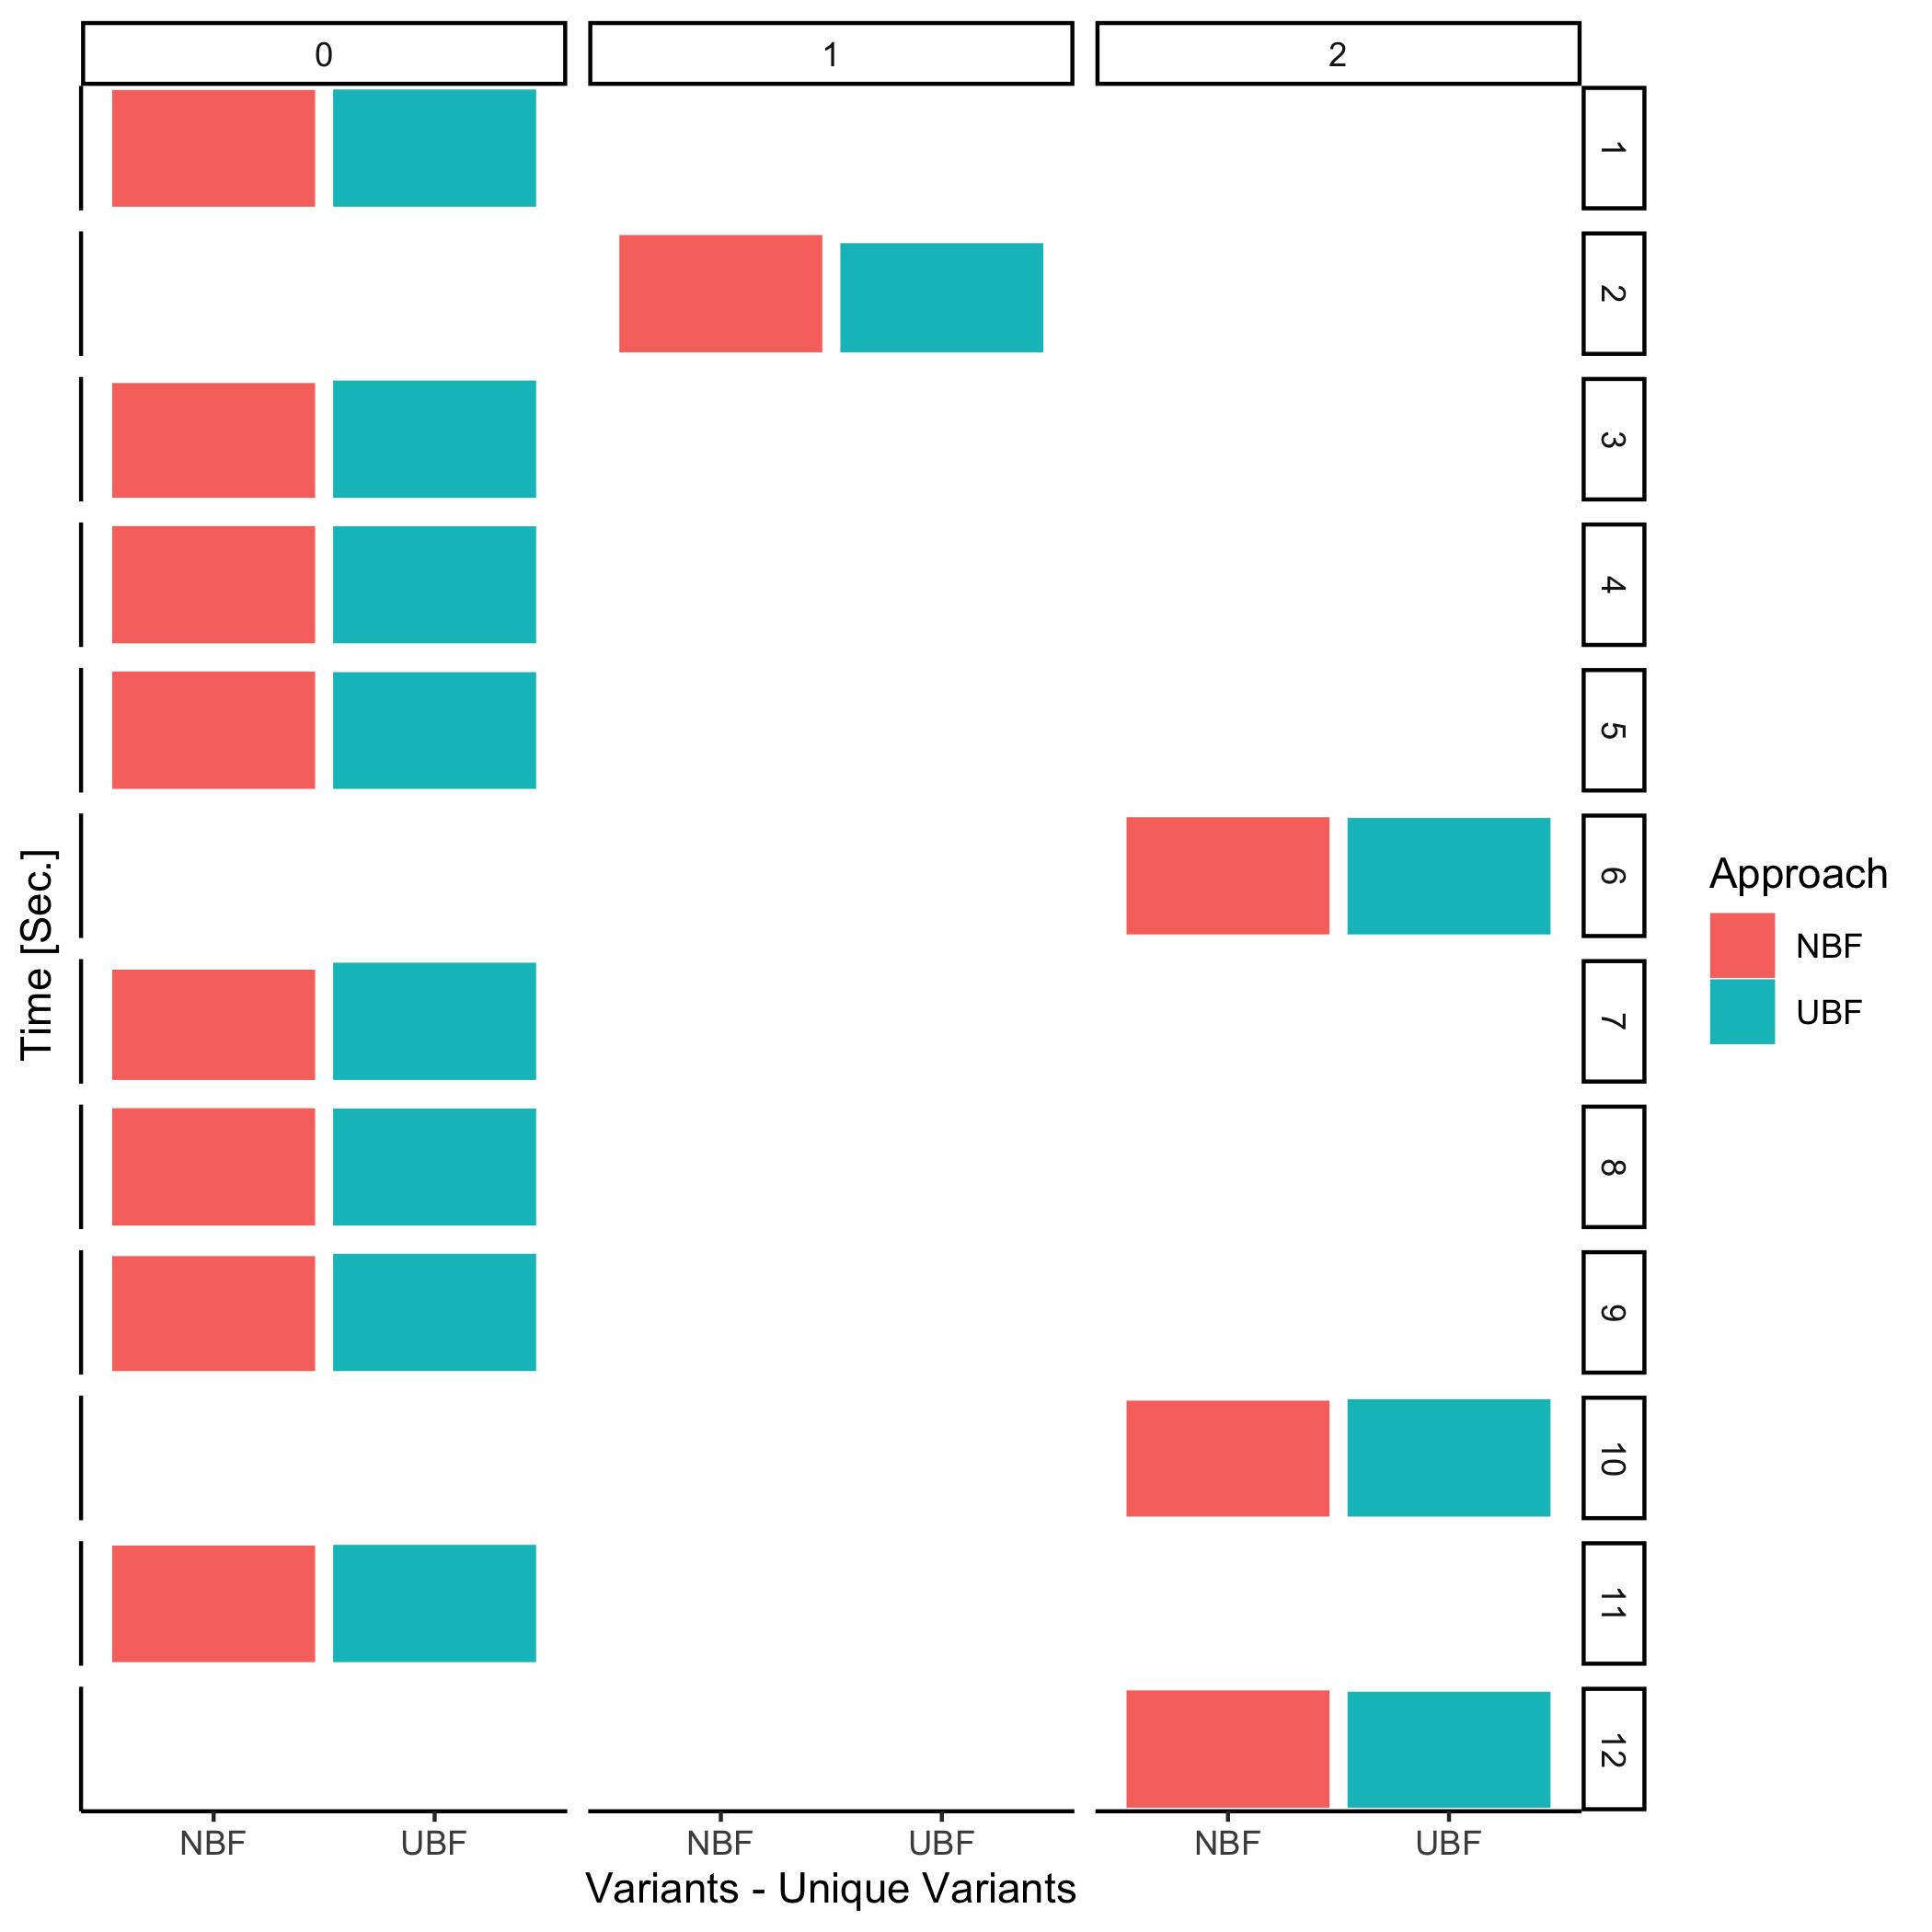
\includegraphics[width=.7\textwidth]{figs/plots/emp-nbf-ubf.png}
\caption{}
\label{fig:sub1}
\end{subfigure}%
\begin{subfigure}{.5\linewidth}
\centering
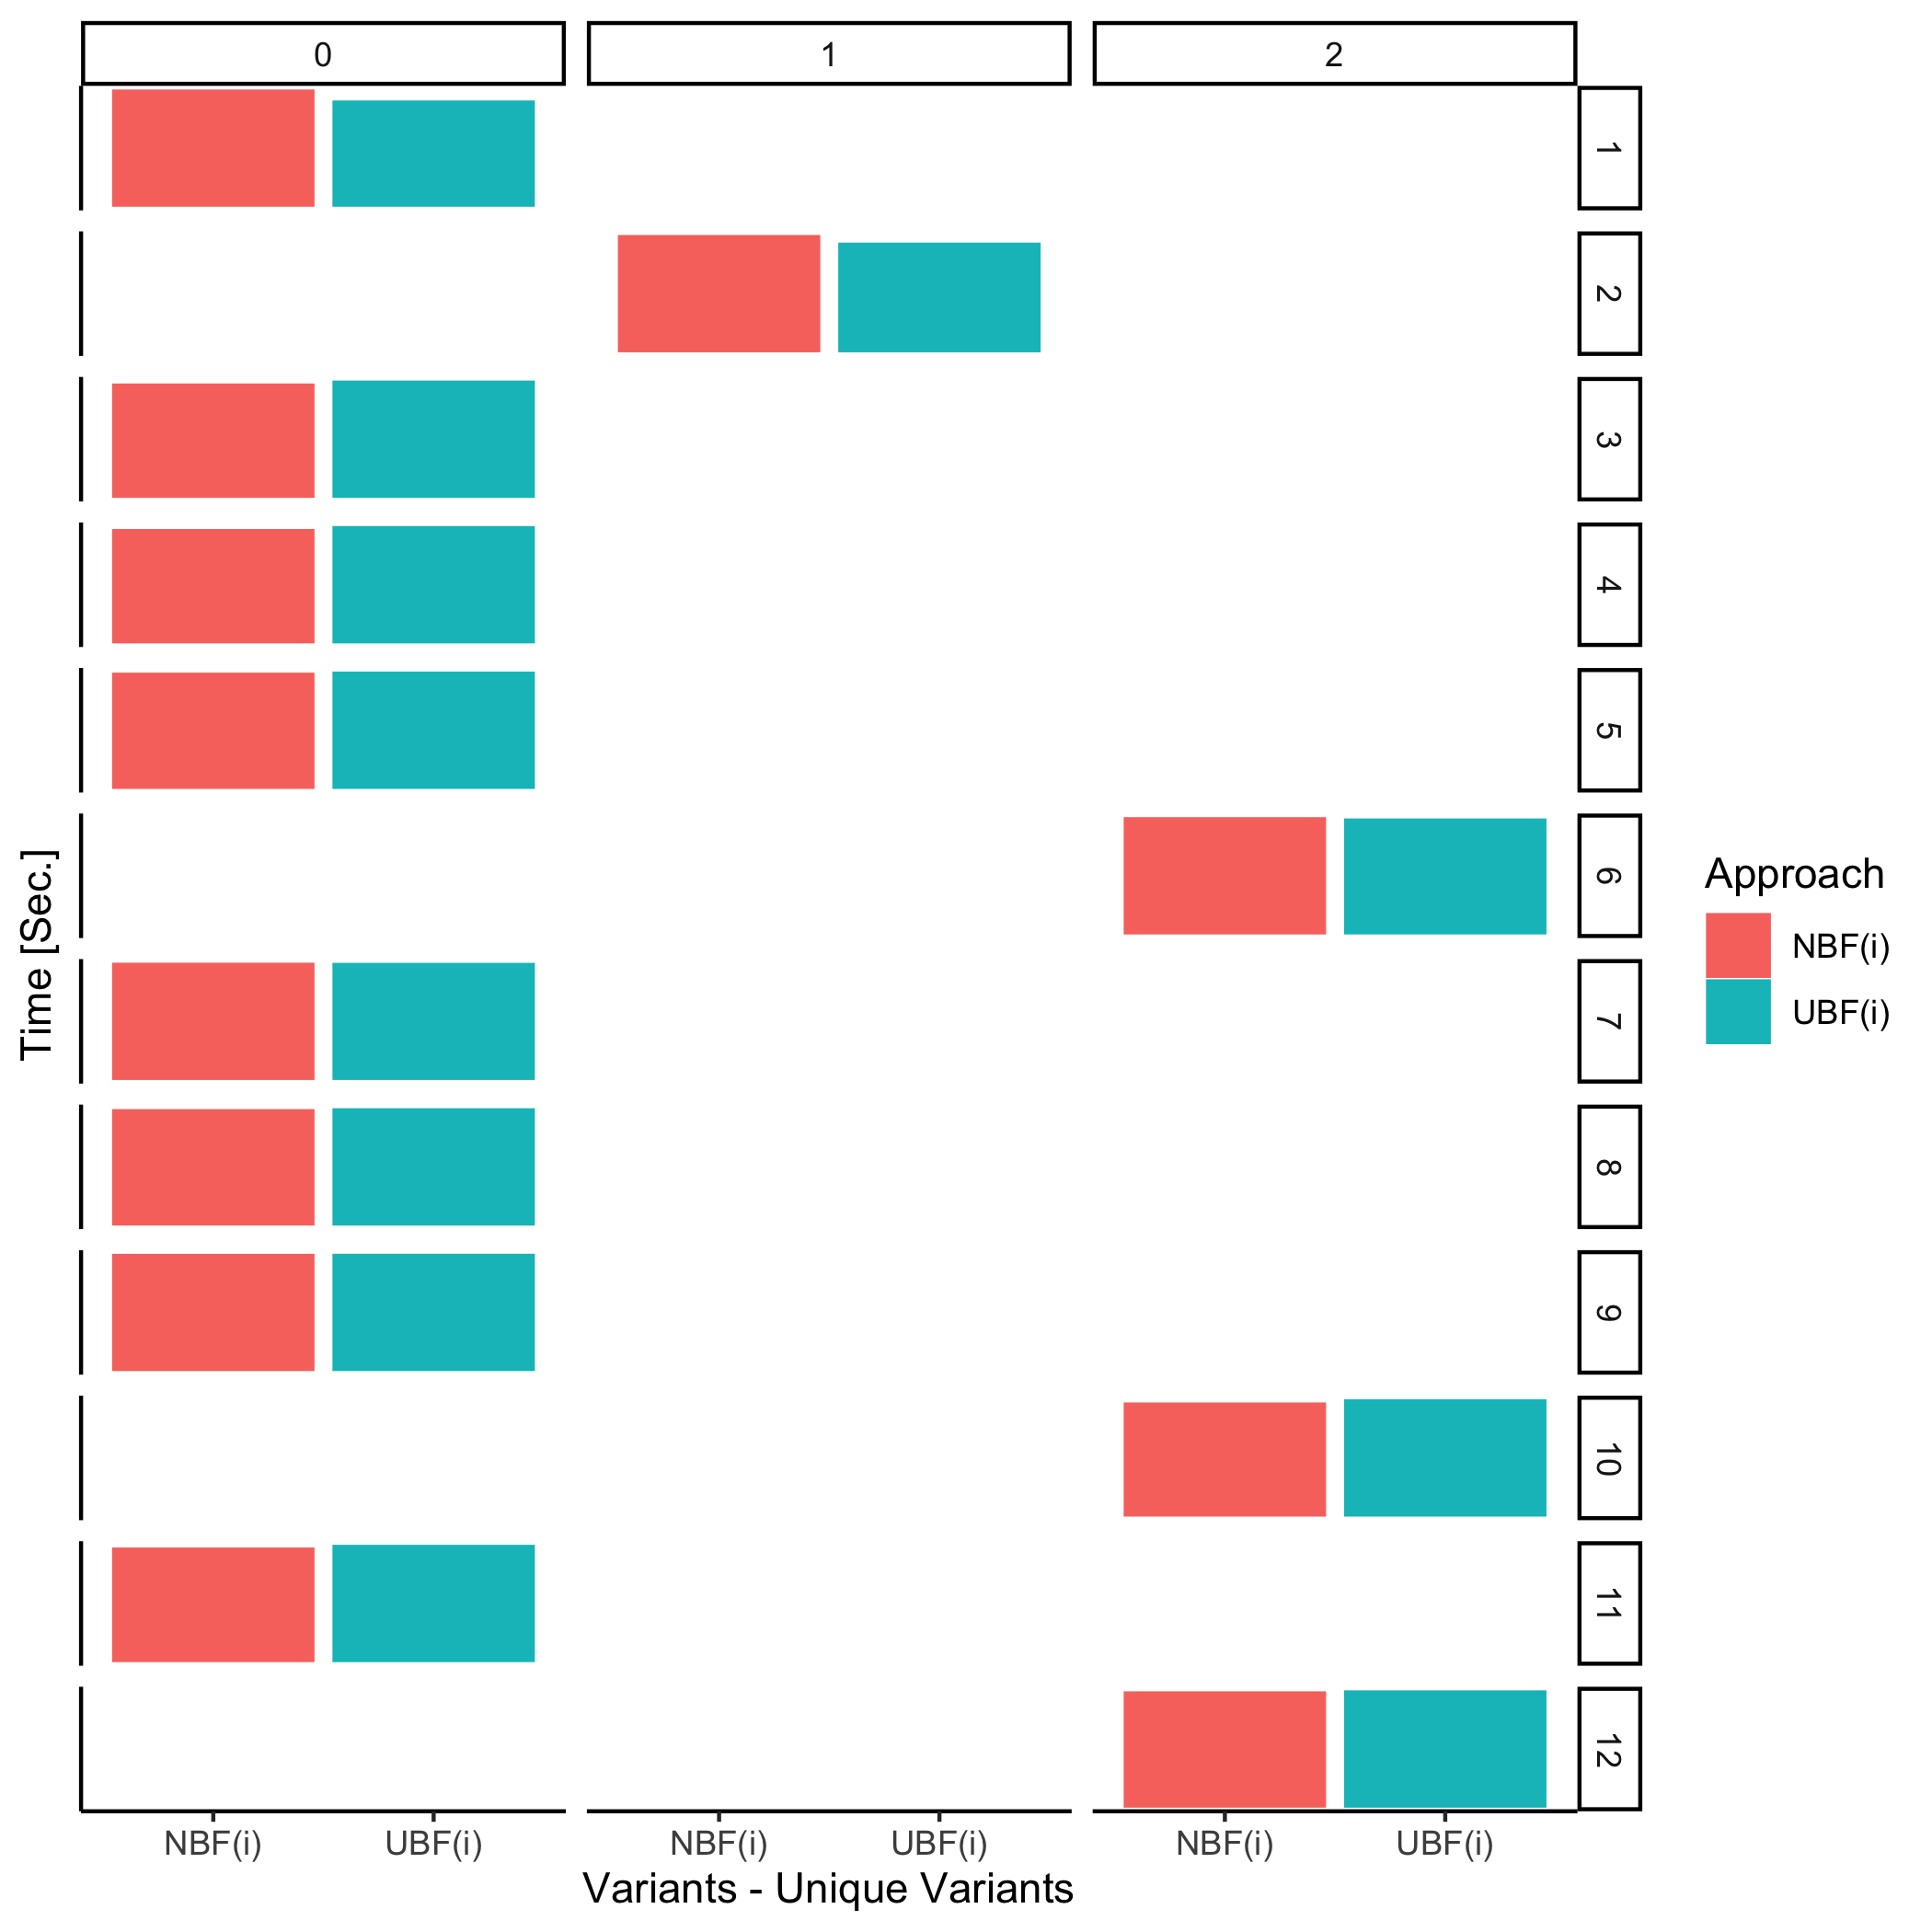
\includegraphics[width=.7\textwidth]{figs/plots/emp-nbfi-ubfi.png}
\caption{}
\label{fig:sub2}
\end{subfigure}\\[1ex]
\begin{subfigure}{0.5\linewidth}
\centering
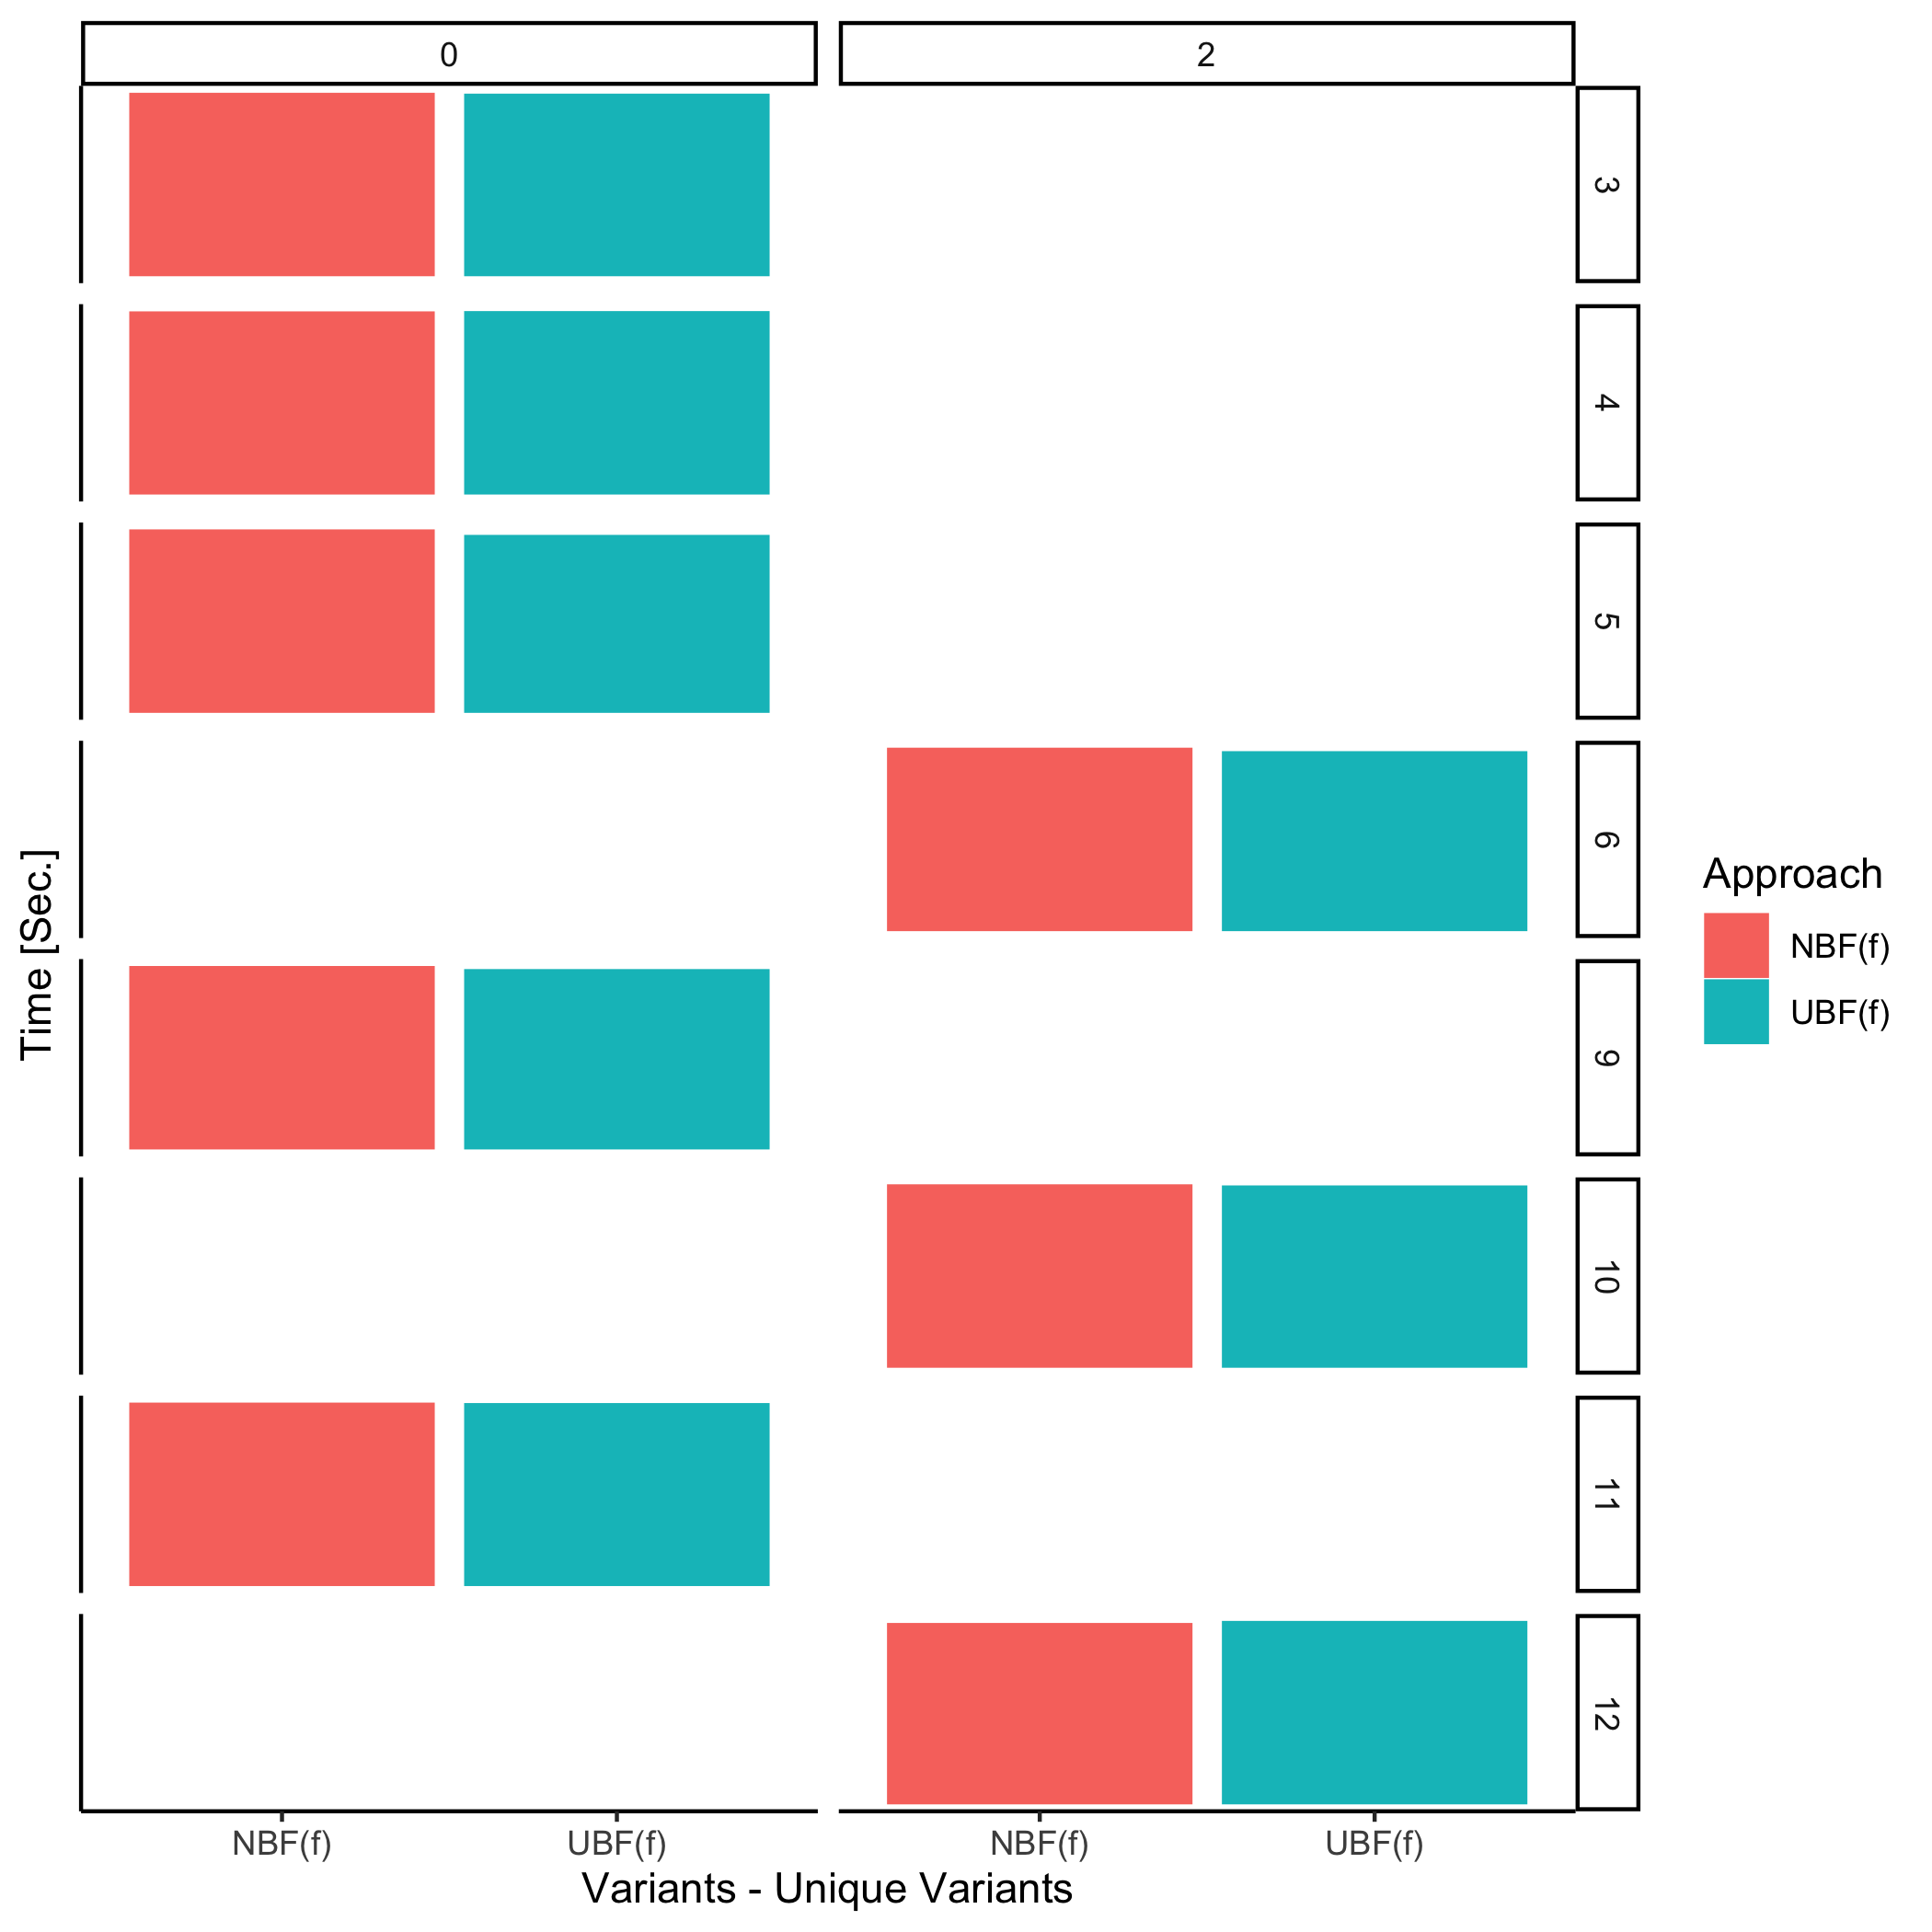
\includegraphics[width=.7\textwidth]{figs/plots/emp-nbff-ubff.png}
\caption{}
\label{fig:sub3}
\end{subfigure}
\begin{subfigure}{0.5\linewidth}
\centering
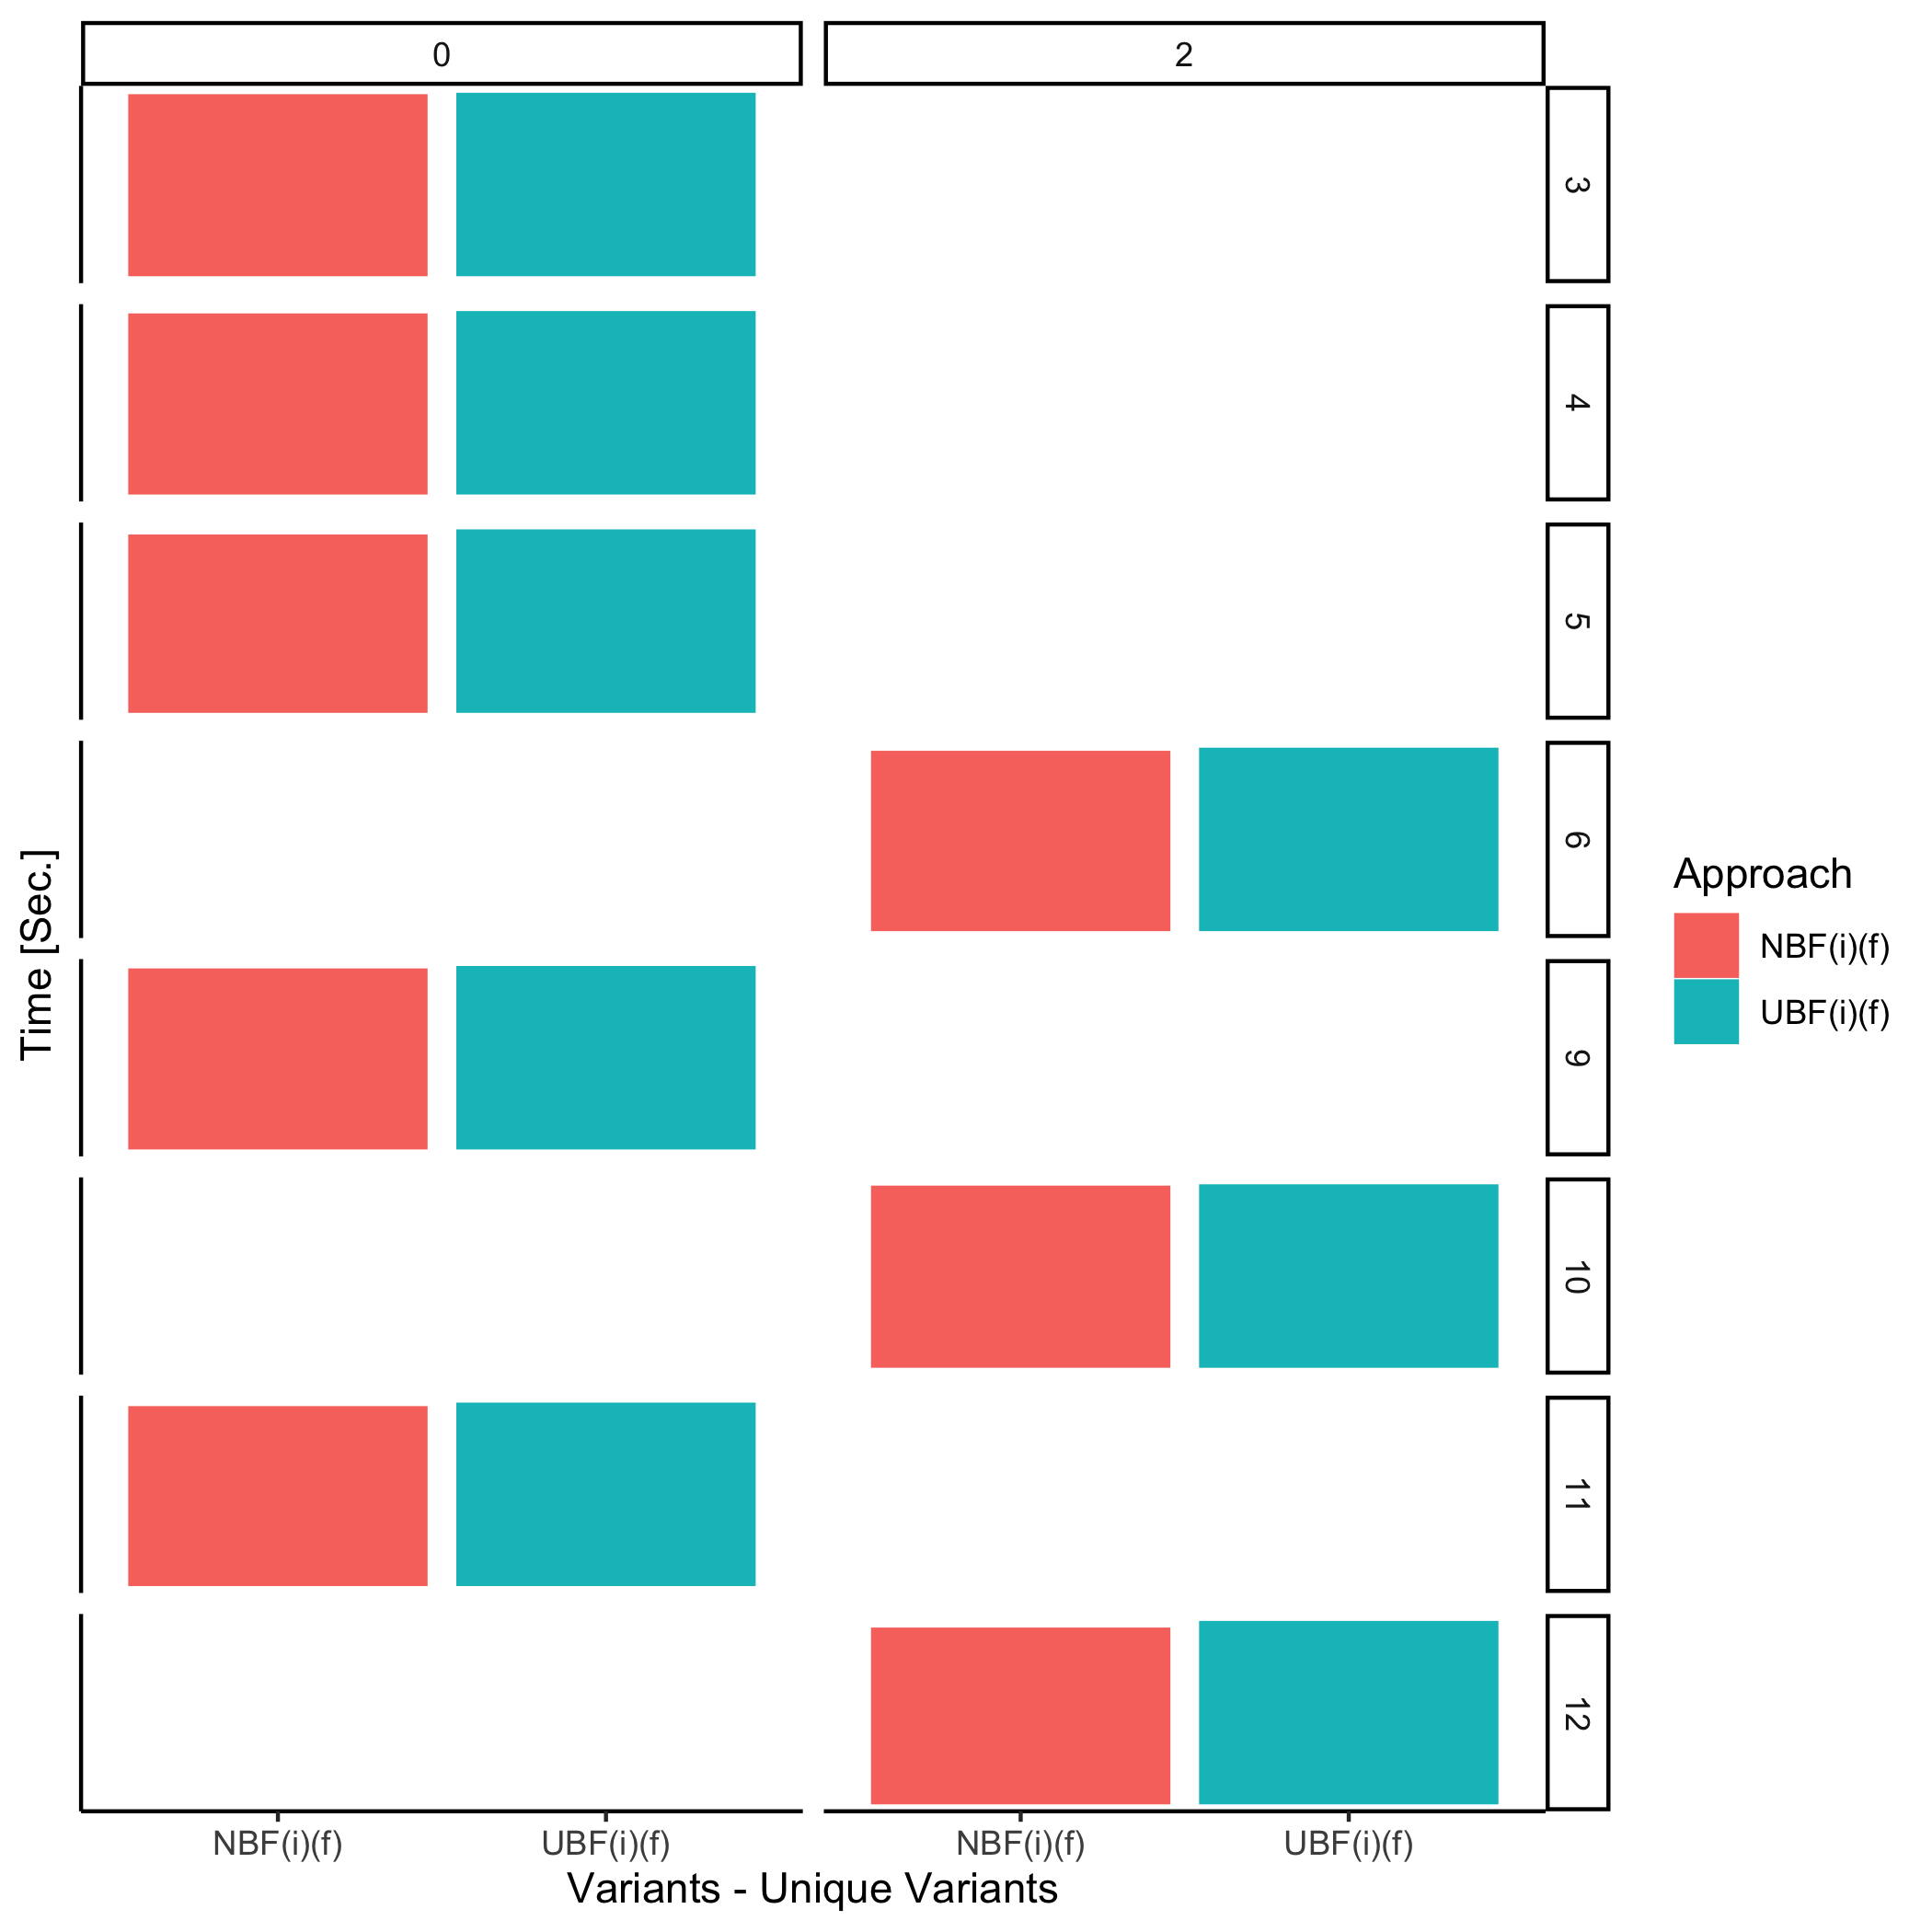
\includegraphics[width=.7\textwidth]{figs/plots/emp-nbfif-ubfif.png}
\caption{}
\label{fig:sub4}
\end{subfigure}
\caption{Three subfigures}
\label{fig:test}
\end{figure}

\begin{figure*}[t!]
    \centering
    \begin{subfigure}[t]{0.5\textwidth}
        \centering
        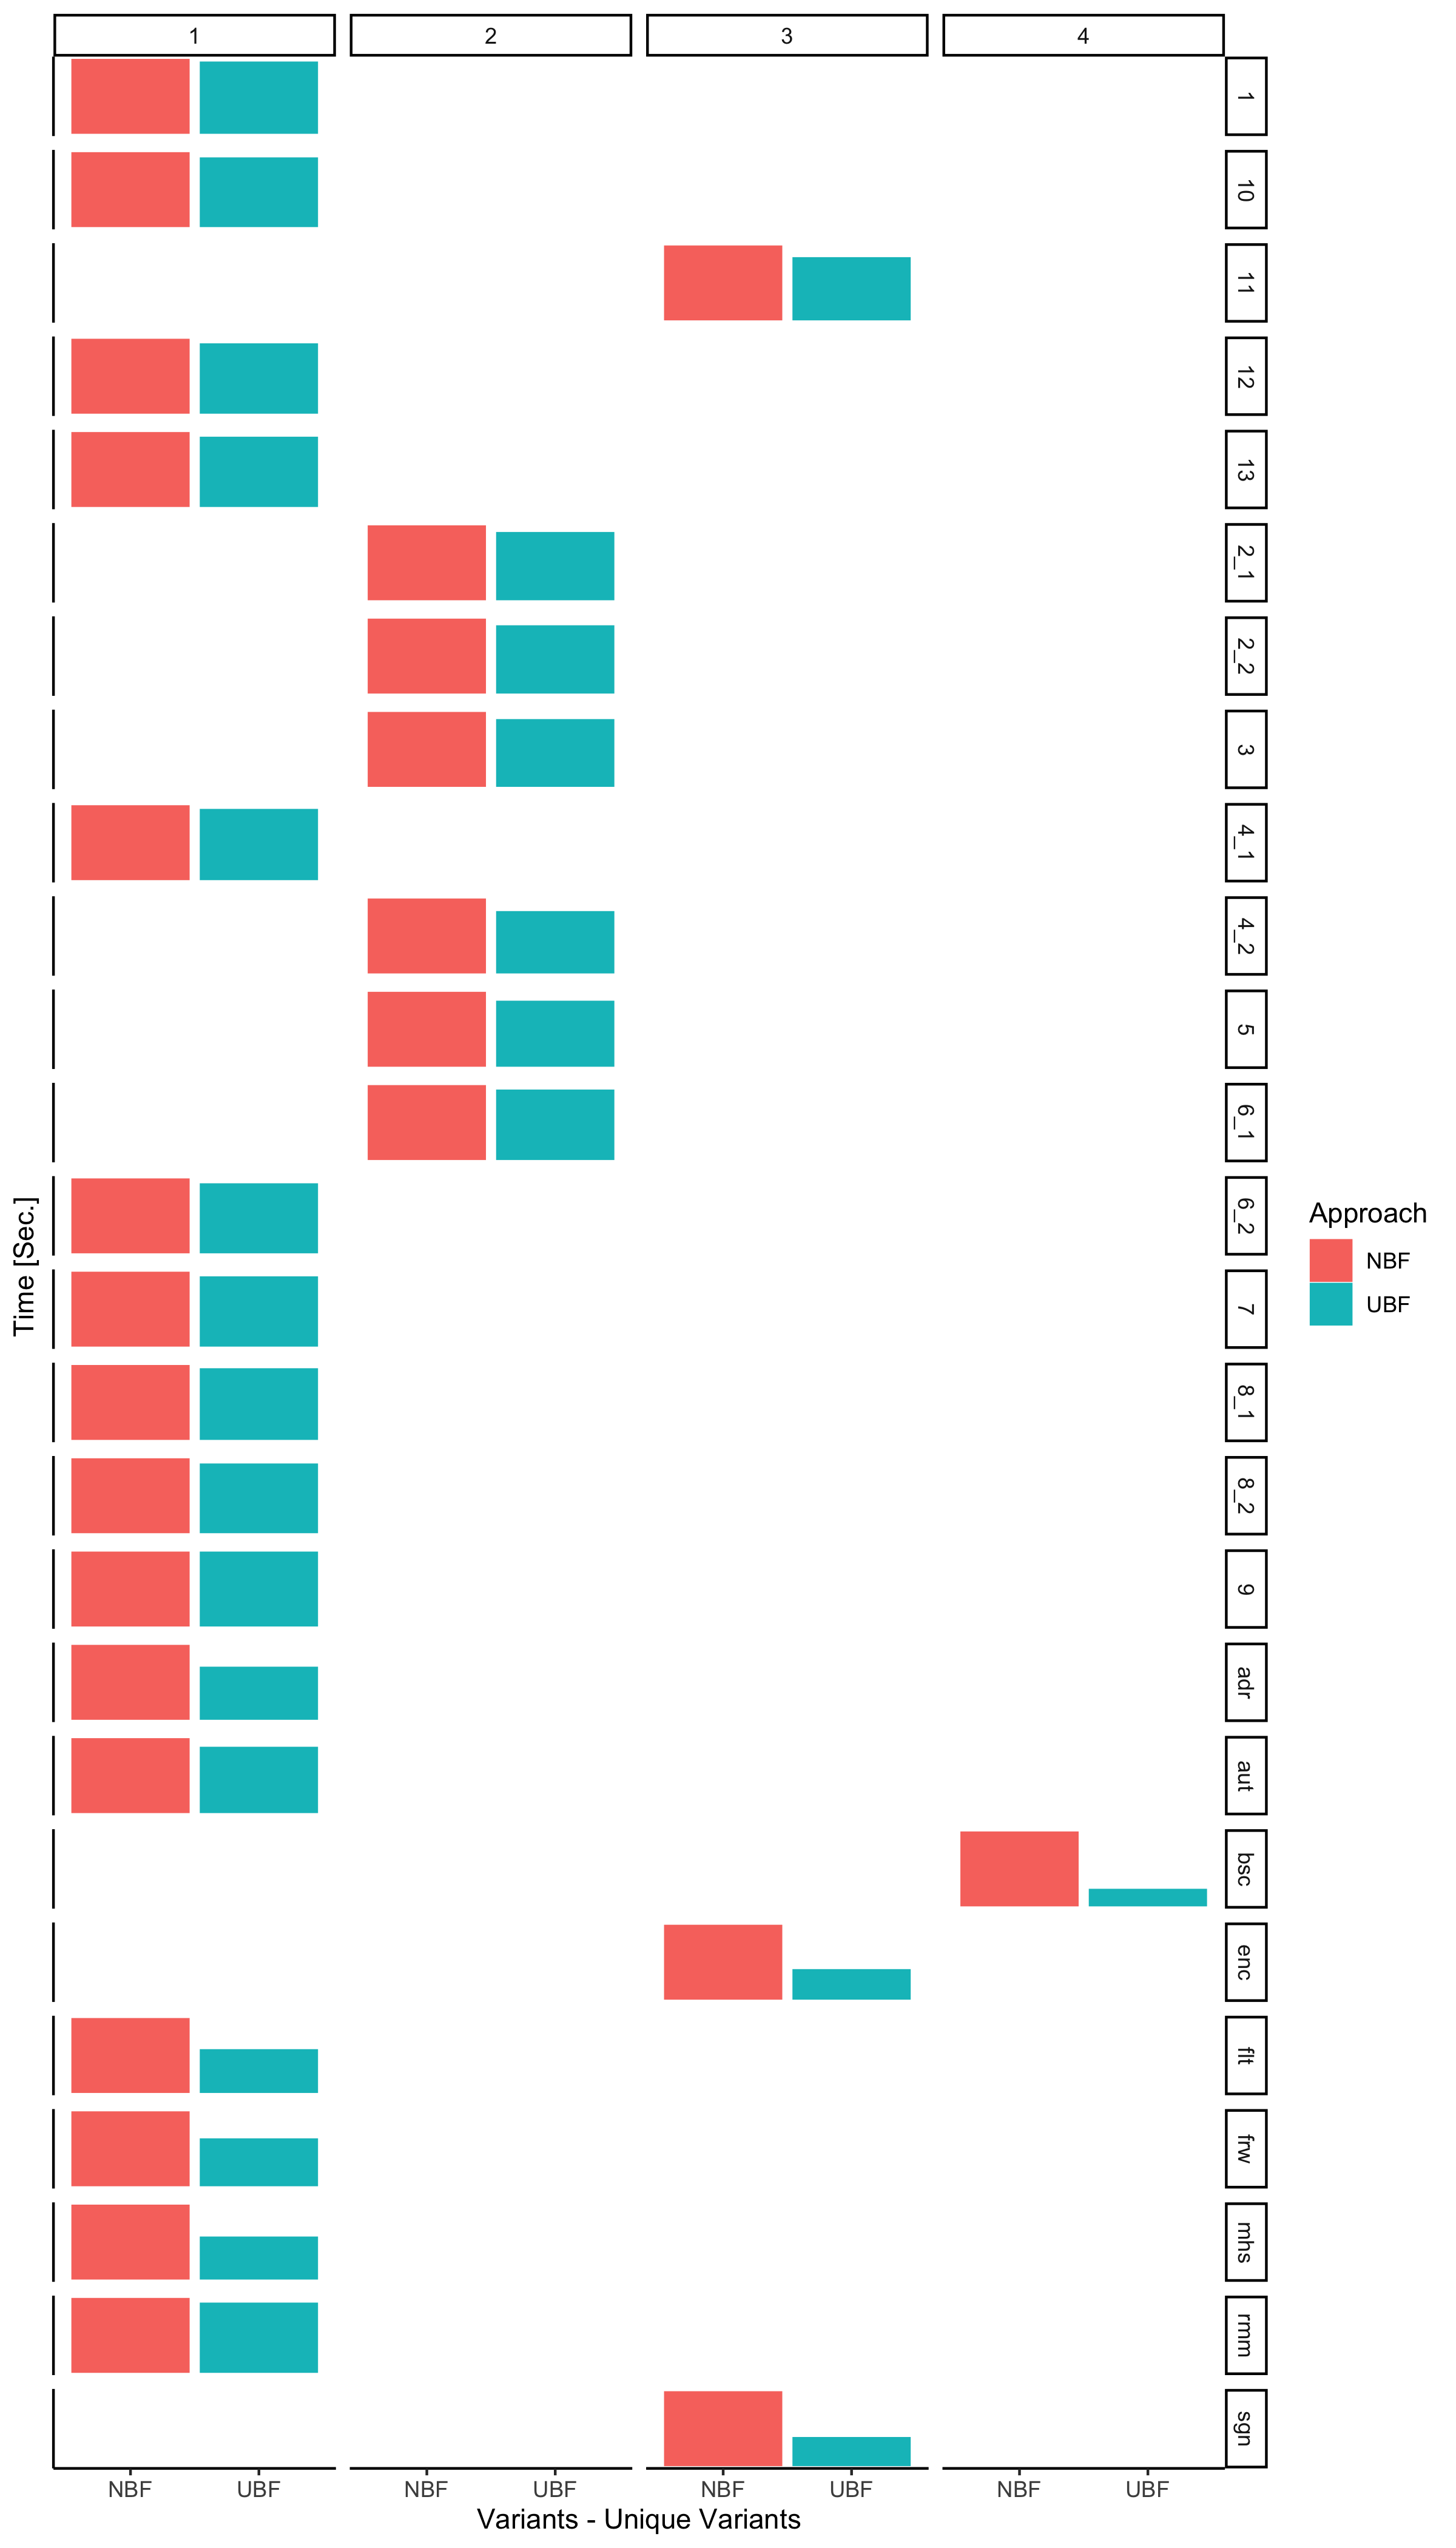
\includegraphics[scale=0.09]{figs/plots/enron-nbf-ubf.png}
        \caption{Lorem ipsum}
    \end{subfigure}%
    ~ 
    \begin{subfigure}[t]{0.5\textwidth}
        \centering
        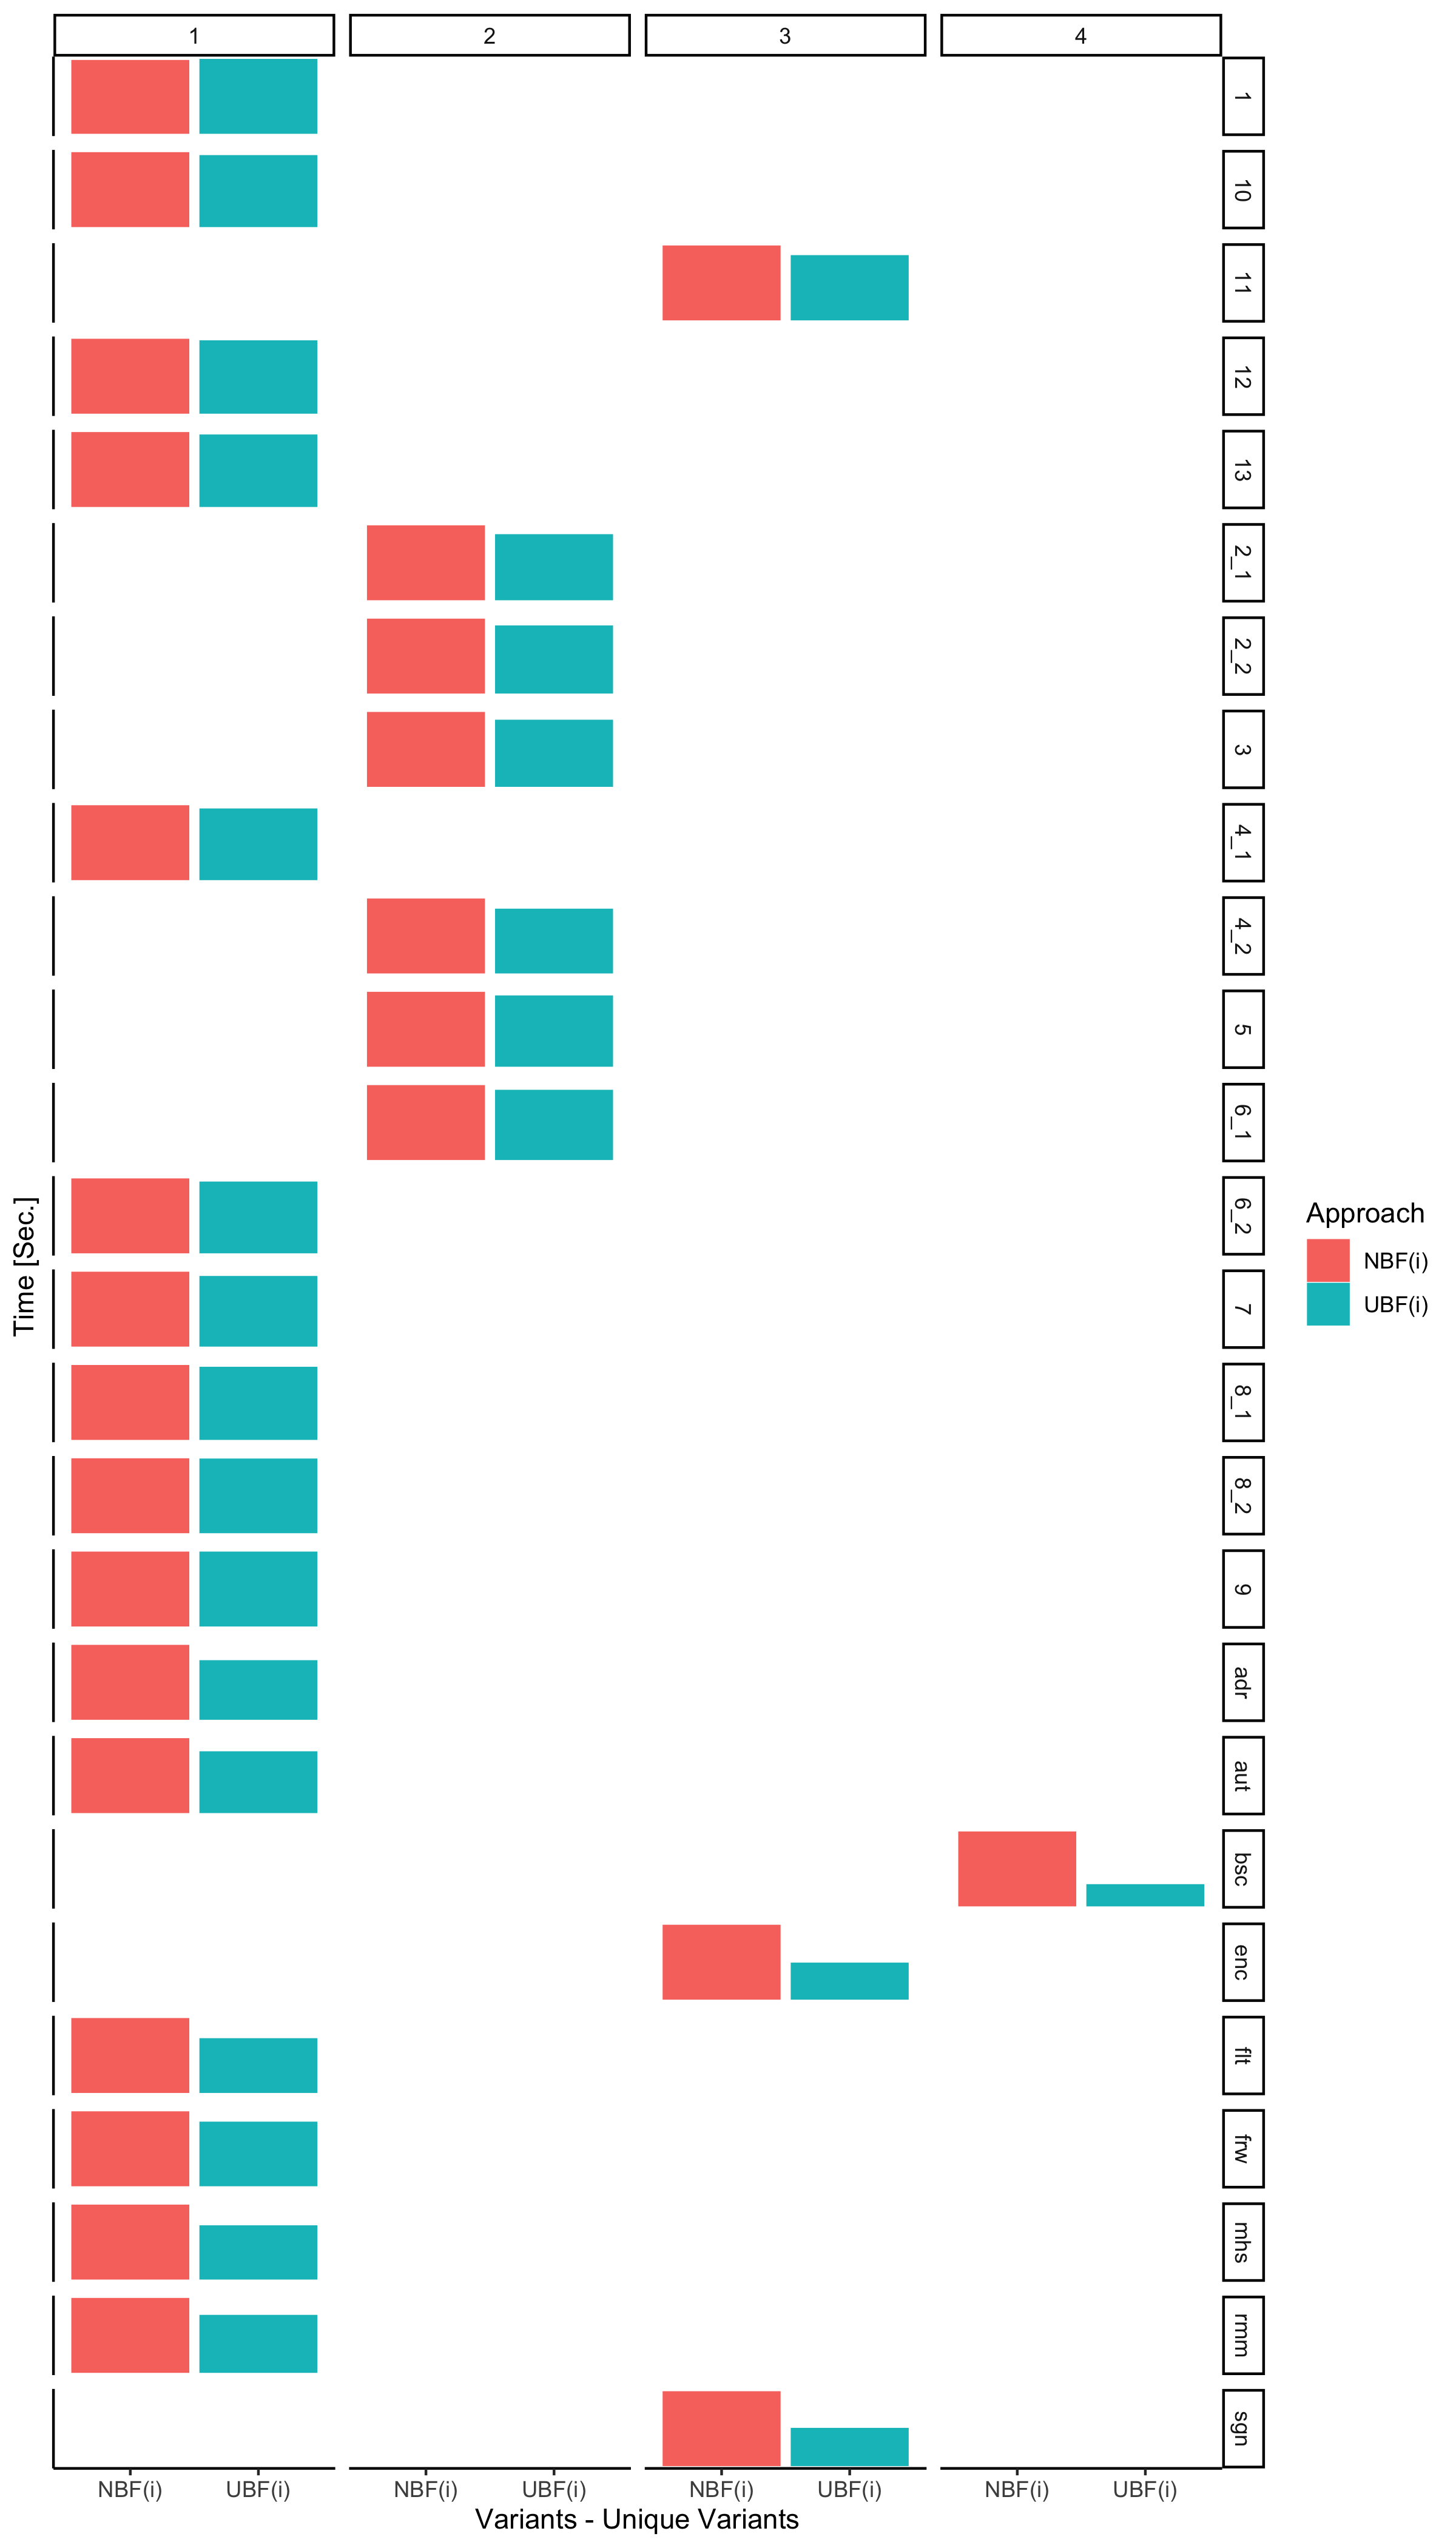
\includegraphics[scale=0.09]{figs/plots/enron-nbfi-ubfi.png}
        \caption{Lorem ipsum, lorem ipsum,Lorem ipsum, lorem ipsum,Lorem ipsum}
    \end{subfigure}
    \caption{Caption place holder}
\end{figure*}

